\documentclass[12pt]{article}
\usepackage[english]{babel}
\usepackage{natbib}
\usepackage{url}
\usepackage[utf8x]{inputenc}
\usepackage{amsmath}
\usepackage{graphicx}
\graphicspath{{images/}}
\usepackage{parskip}
\usepackage{fancyhdr}
\usepackage{vmargin}
\usepackage{xcolor}
\usepackage{siunitx}
\usepackage{physics}
\setmarginsrb{3 cm}{2 cm}{3 cm}{2 cm}{1 cm}{1.5 cm}{1 cm}{1.5 cm}

\title{Lab 06}													% Title
\author{G 03}														% Author
\date{14 may 2019}														% Date

\makeatletter
\let\thetitle\@title
\let\theauthor\@author
\let\thedate\@date
\makeatother

\pagestyle{fancy}
\fancyhf{}
\rhead{\theauthor}
\lhead{\thetitle}
\cfoot{\thepage}
\newcommand{\mis}[3]{(#1 \pm #2) \ #3}
\newcommand{\misp}[3]{(#1 \#3 \pm #2}
\begin{document}

%%%%%%%%%%%%%%%%%%%%%%%%%%%%%%%%%%%%%%%%%%%%%%%%%%%%%%%%%%%%%%%%%%%%%%%%%%%%%%%%%%%%%%%%%

\begin{titlepage}
	\centering
    \vspace*{0.5 cm}
    
\includegraphics[scale = 0.75]{polito.jpg}\\[1.0 cm]				% University Logo
    \textsc{\LARGE Politecnico di Torino}\\[2.0 cm]						% University Name
	\textsc{\Large Digital systems electronics\\ A.A. 2018/2019}\\[0.5 cm]		% Course Code
	\textsc{\Large Prof. G. Masera}\\[0.5 cm]		% Nome del Professore
	\rule{\linewidth}{0.2 mm} \\[0.4 cm]
	{ \huge \bfseries \thetitle \\ \small \thedate}\\
	\rule{\linewidth}{0.2 mm} \\[1.5 cm]
	
	\begin{minipage}{0.4\textwidth}
		\begin{flushleft} \large
			Berchialla Luca\\												%Cognomi e nomi
			Laurasi Gjergji
			\\
			
			Mattei Andrea\\
            Lombardo Domenico Maria\\
            
			\end{flushleft}
			\end{minipage}~
			\begin{minipage}{0.4\textwidth}
            
			\begin{flushright} \large
			236032\\													%Matricole
			238259\\
            233755\\
            233959\\
            
		\end{flushright}
        
	\end{minipage}\\[2 cm]
	
\end{titlepage}

%%%%%%%%%%%%%%%%%%%%%%%%%%%%%%%%%%%%%%%%%%%%%%%%%%%%%%%%%%%%%%%%%%%%%%%%%%%%%%%%%%%%%%%%%
\newpage

\section*{Introduction to the assigned problem}
This relation deals with the design of a simple digital filter. From the given functional specifications, a final digital circuit has been implemented in VHDL including memories, control unit and data-path. 
\newline The design process will be analyzed using  a bottom-up approach, starting from the individual components and their interconnections to the final custom designed FSM.





\section*{Overall specs description}

As already mentioned, the final  purpose of this activity is to implement a digital filter following the relation:
\[Y(n) = -0.5X(n) - 2X(n-1) + 4X(n-2) + 0.25X(n-3) \]

where $ X(n) $ are the input stream data and $ Y(n) $ the corresponding filtered data generated by the top equation.

The circuit starts by means of a $START$ signal which enable a loading process of the input data into a 1 kByte memory. Then, the circuit automatically filters the data stream exploiting the equation already provided and loads the output filtered data into a second memory. Finally, the circuit reports end of process asserting an $HIGH$ logical value to the $DONE$ signal and awaits until the next $START$.

Every used component will now be discussed as single blocks, and individually debugged:
\newpage
\subsection*{Memories}

As already discussed, the final implementation will save the input data in a 1kByte memory while memorizing the output data into an output memory. 


\begin{figure}[h]
	\centering
	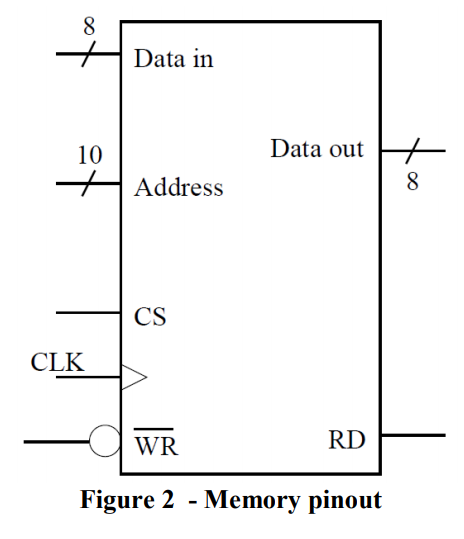
\includegraphics[scale = 0.7]{immagini/memory.png}
	\caption{ 1kByte memory }
\end{figure}

The memories store 1024 samples represented as 8 bit wide 2's complement values.
The writing operation is synchronous with the positive edge of the clock, while the reading is asynchronous. 

The samples must be stored in order, from address 0 to 1023.

Once the desired address is selected and the RD signal asserted, the output data are shown in the $ data out $ parallel output.

The figure below shows the testbench for the register file.
\newline\newline\newline
\begin{figure}[h]
	\centering
	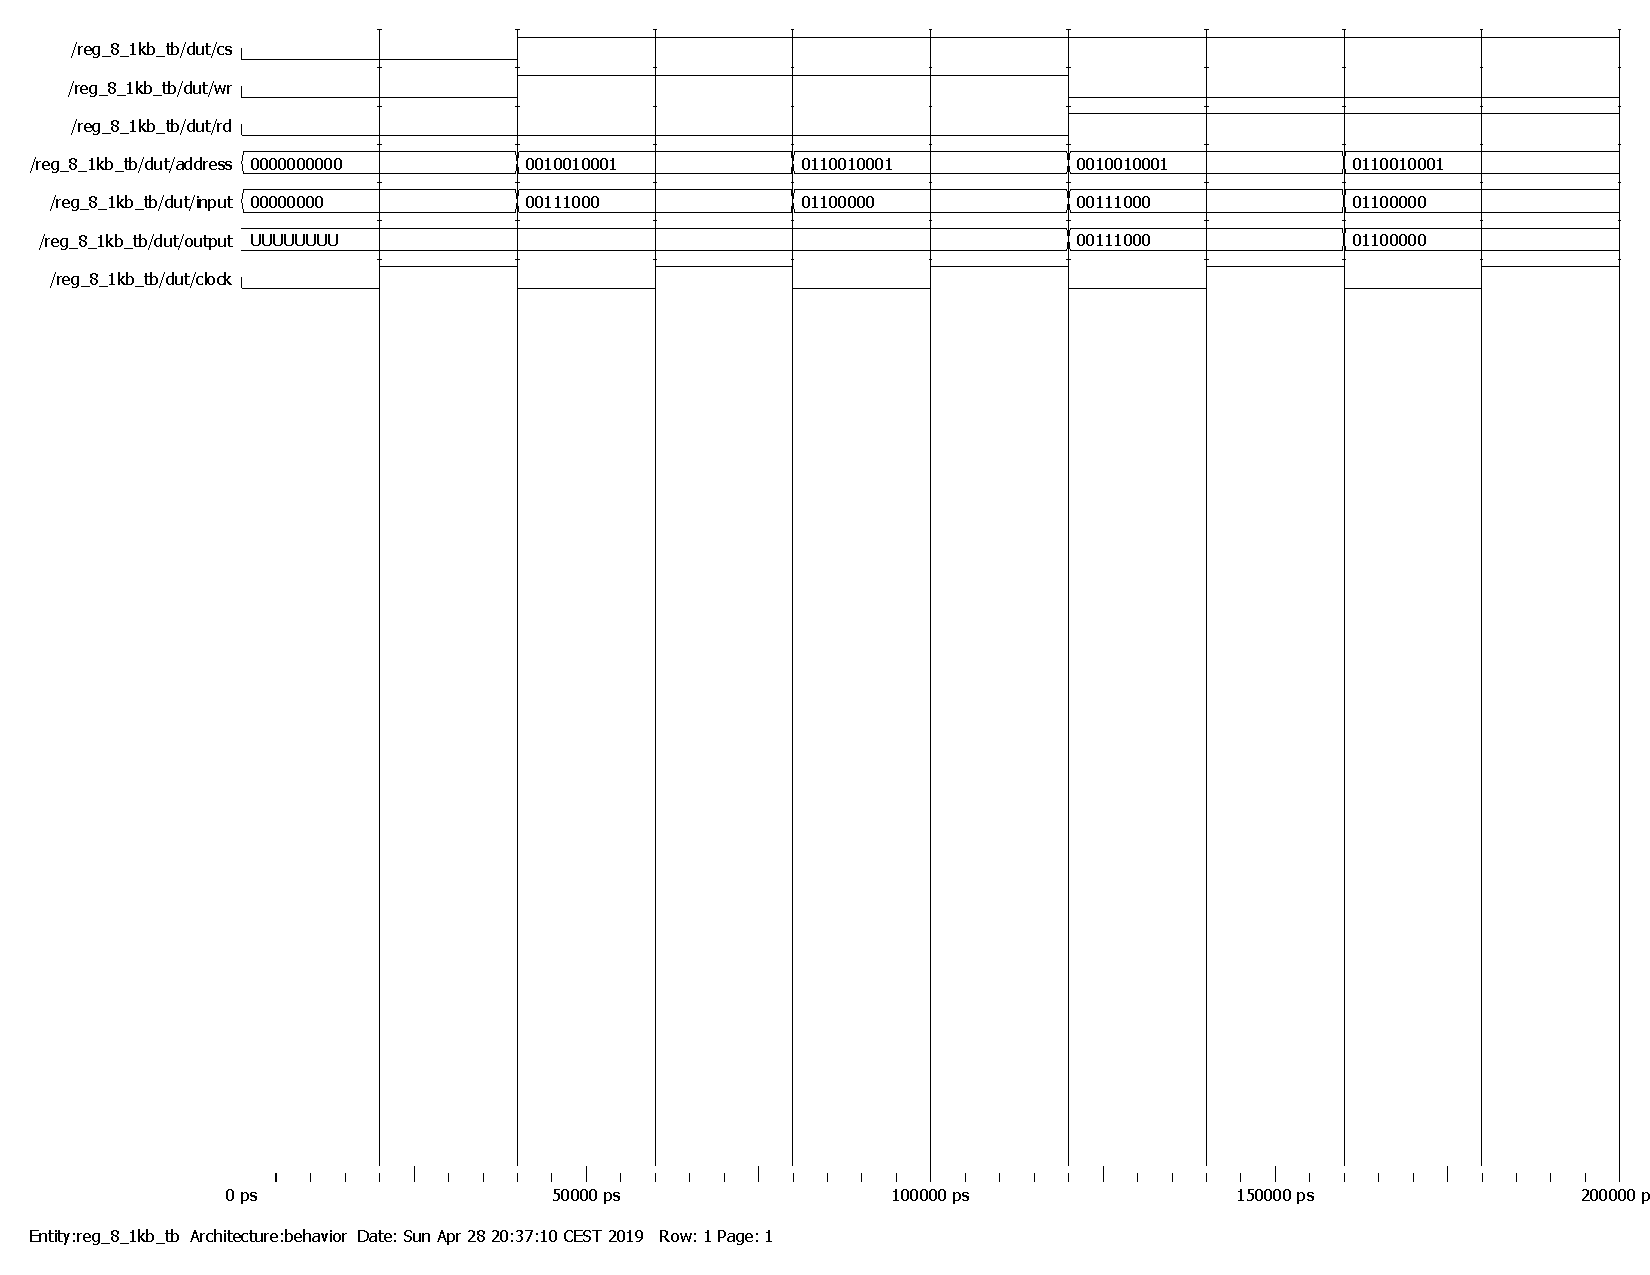
\includegraphics[scale = 0.55]{immagini/memory_tb.png}
	\caption{Memory testbench}
\end{figure}

\newpage
\subsection*{Shift registers and registers}

To be able to implement the already stated main equation, the circuit needs to perform 2s multiple multiplication and/or division.

The final implementation exploits the left and right shifting operations.

A 11 bit shift register has been implemented with parallel load and parallel output.

The $LOAD$ signal must be asserted to load the $parallel\;input$ data into the register, in a synchronous way with the positive edge of the clock.

The $SL$ and $SR$ commands permit the left or right shift of the internal memorized data.  
  

\begin{figure}[h]
	\centering
	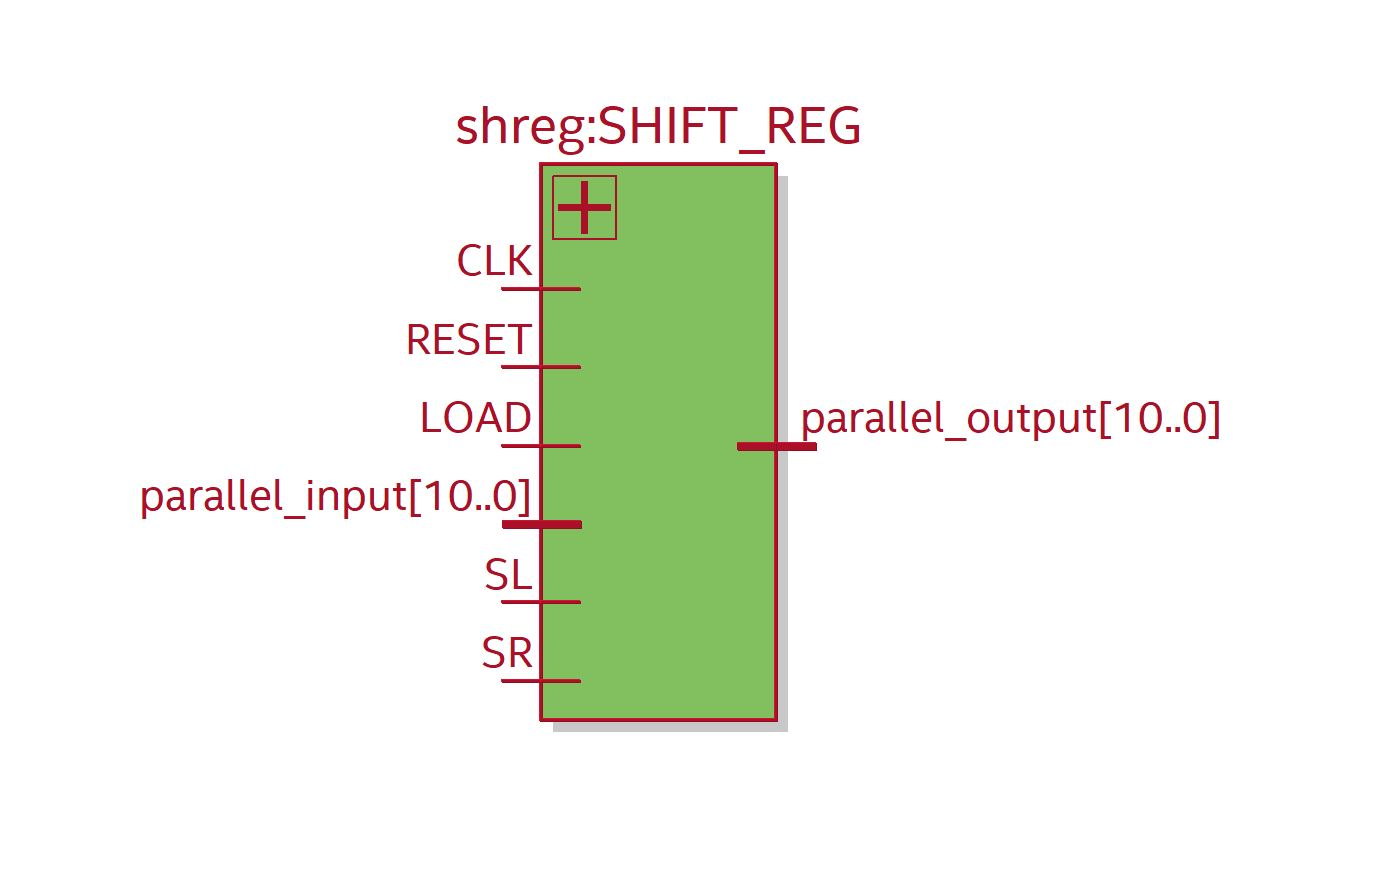
\includegraphics[scale = 0.6]{immagini/shreg.jpg}
	\caption{Shift register}
\end{figure}

The testbench for the 8-bit version is shown below:
 
\begin{figure}[h]
	\centering
	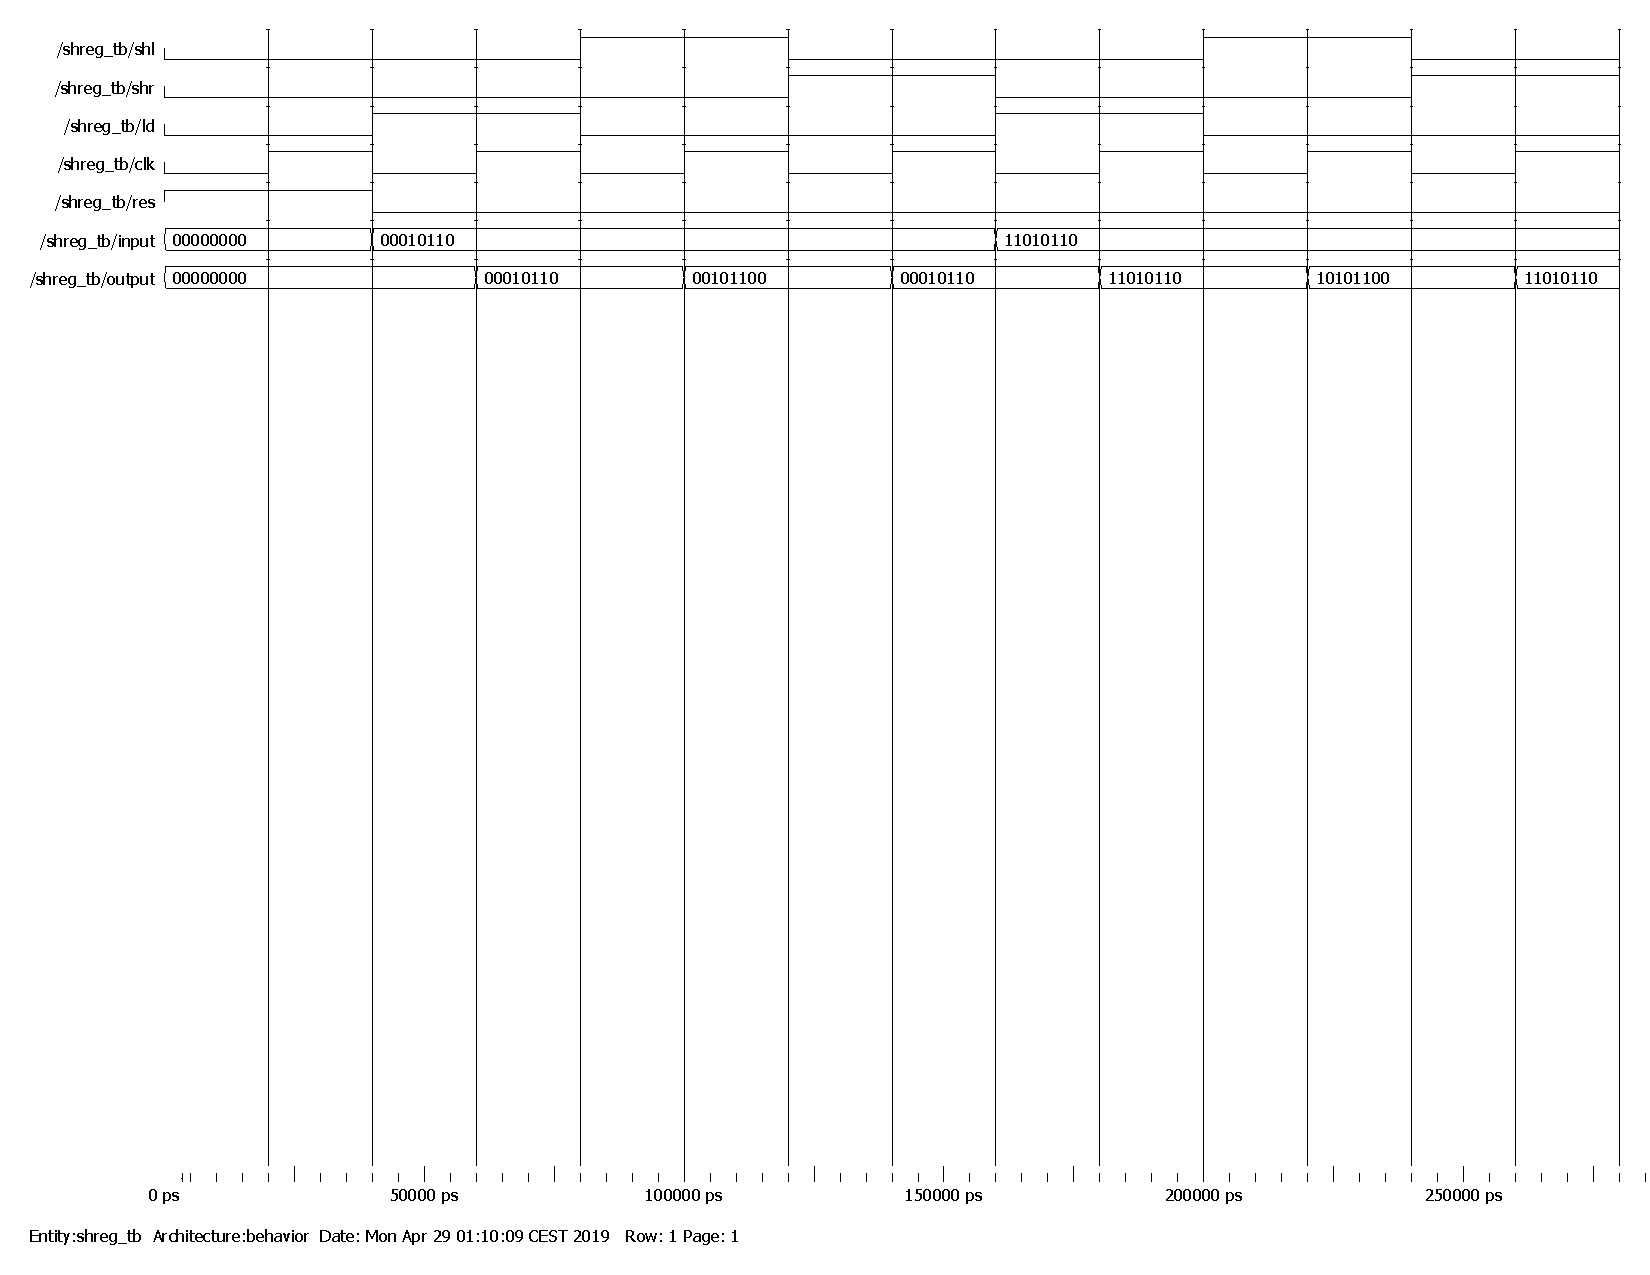
\includegraphics[scale = 0.55]{immagini/shift_reg_tb.png}
	\caption{Shift register test bench}
\end{figure}

\newpage

\subsection*{Adder}

An 11-bit of a classical adder has been implemented, allowed to perform additions and subtractions by means of the  $Cin$ signal.
\begin{figure}[h!]
	\centering
	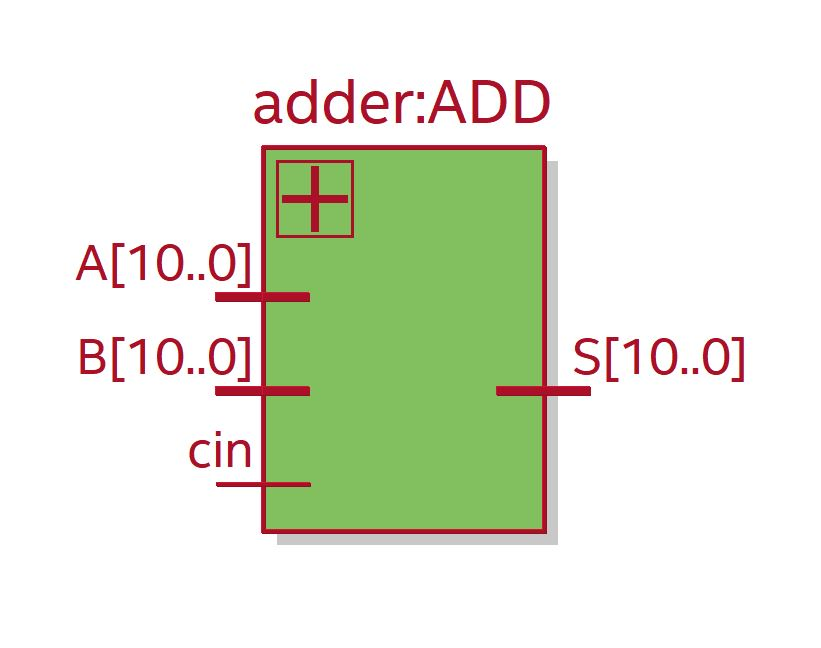
\includegraphics[scale = 0.65]{immagini/adder.jpg}
	\caption{Adder}
\end{figure}


Below is shown the test bench of the designed adder.


\begin{figure}[h]
	\centering
	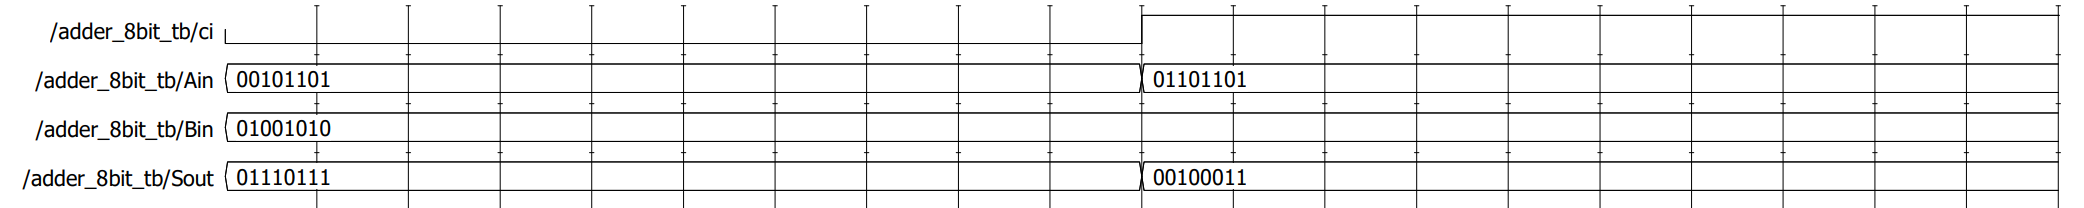
\includegraphics[scale = 0.55]{immagini/adder_tb.png}
	\caption{Adder test bench}
\end{figure}

\subsection*{Data converters}

Finally, since the circuit must be able to determine both overflow and underflow it uses 2 blocks able to convert 8 bit signals to 11 bit and vice versa, as will be discussed in further sections. 

The simulated test bench are shown below: 

\begin{figure}[h!]
	\centering
	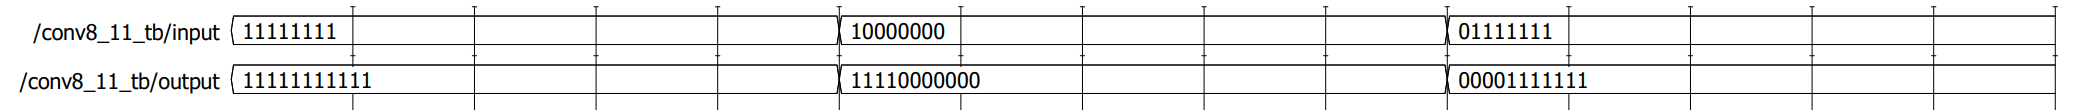
\includegraphics[scale = 0.47]{immagini/8_11_tb.png}
	\vspace{1mm}	
	\centering
	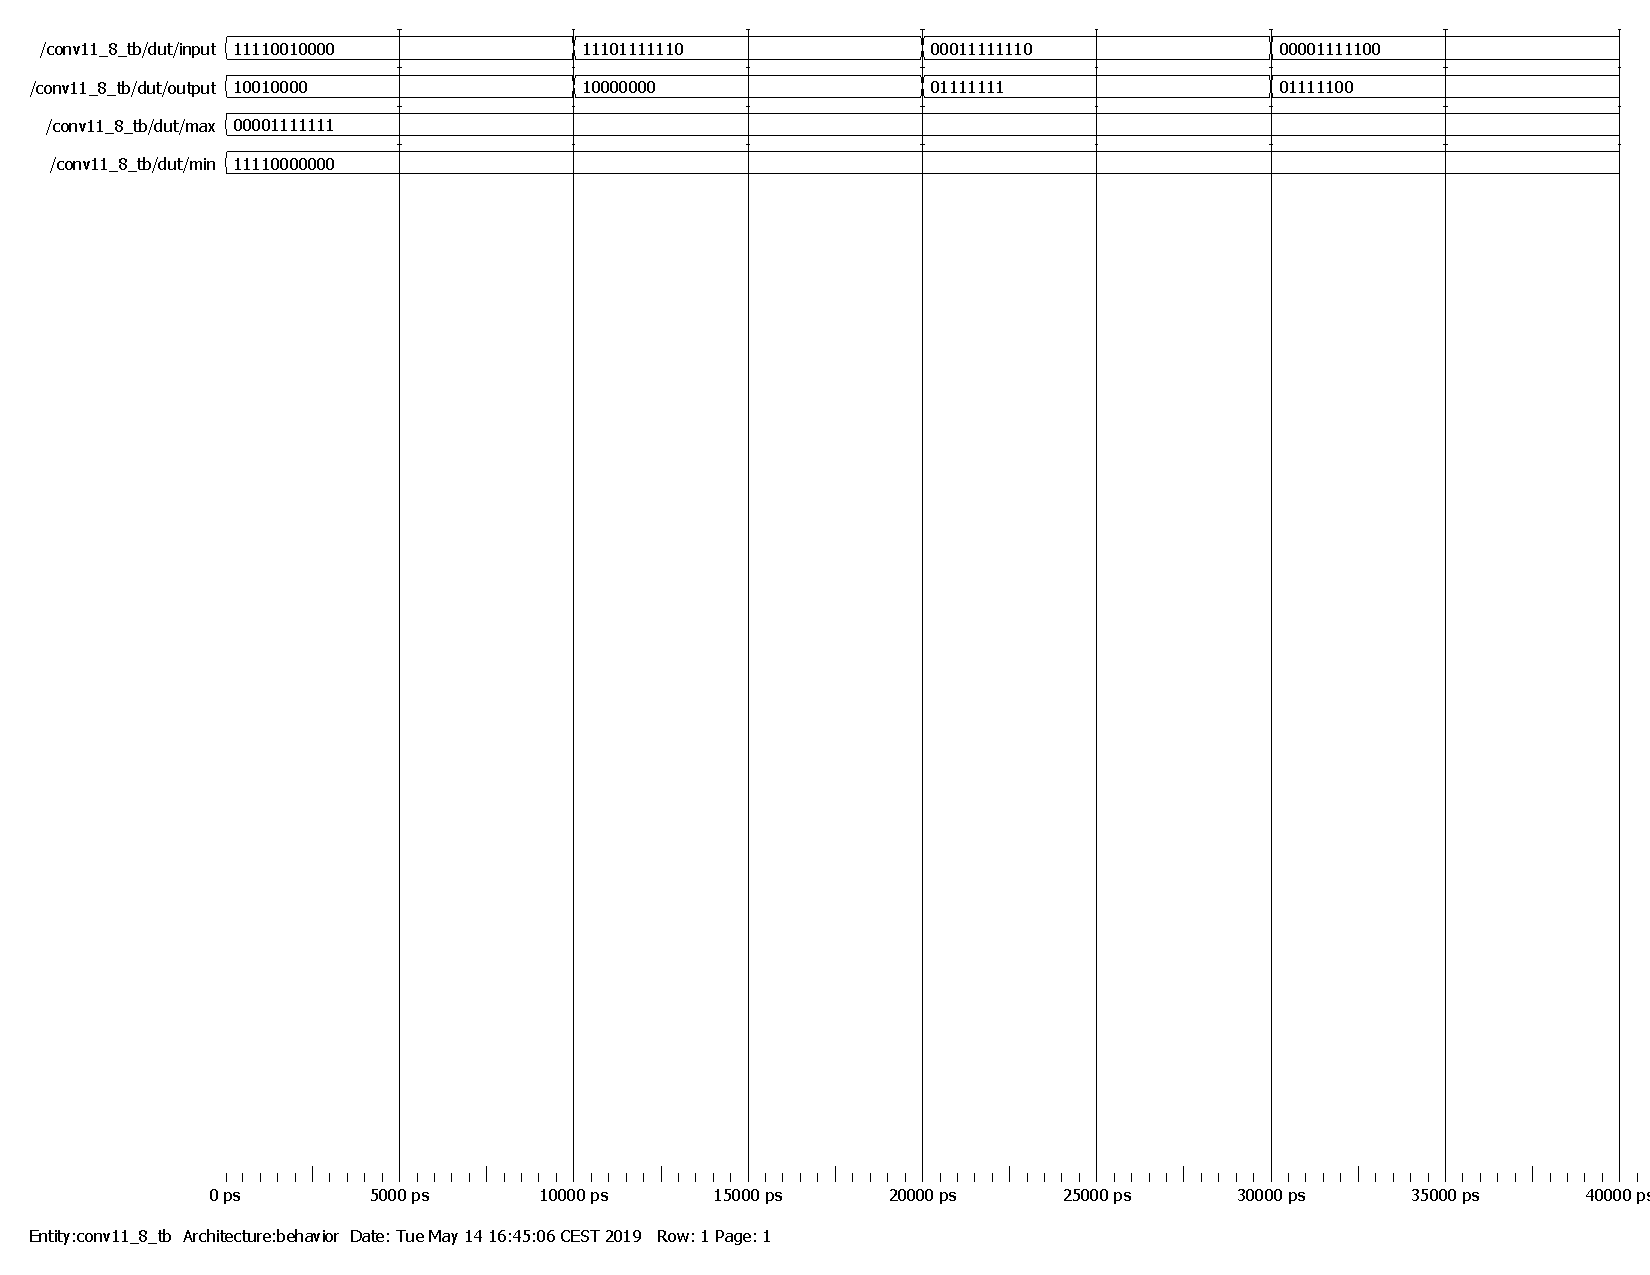
\includegraphics[scale = 0.47]{immagini/11_8_tb.png}
	\caption{8 to 11 bit converter; 11 to 8 bit converter}
\end{figure}
\newpage
\subsection*{Counter}
To be able to go through the various addresses an universal counter has also been implemented as shown: 
\begin{figure}[h!]
	\centering
	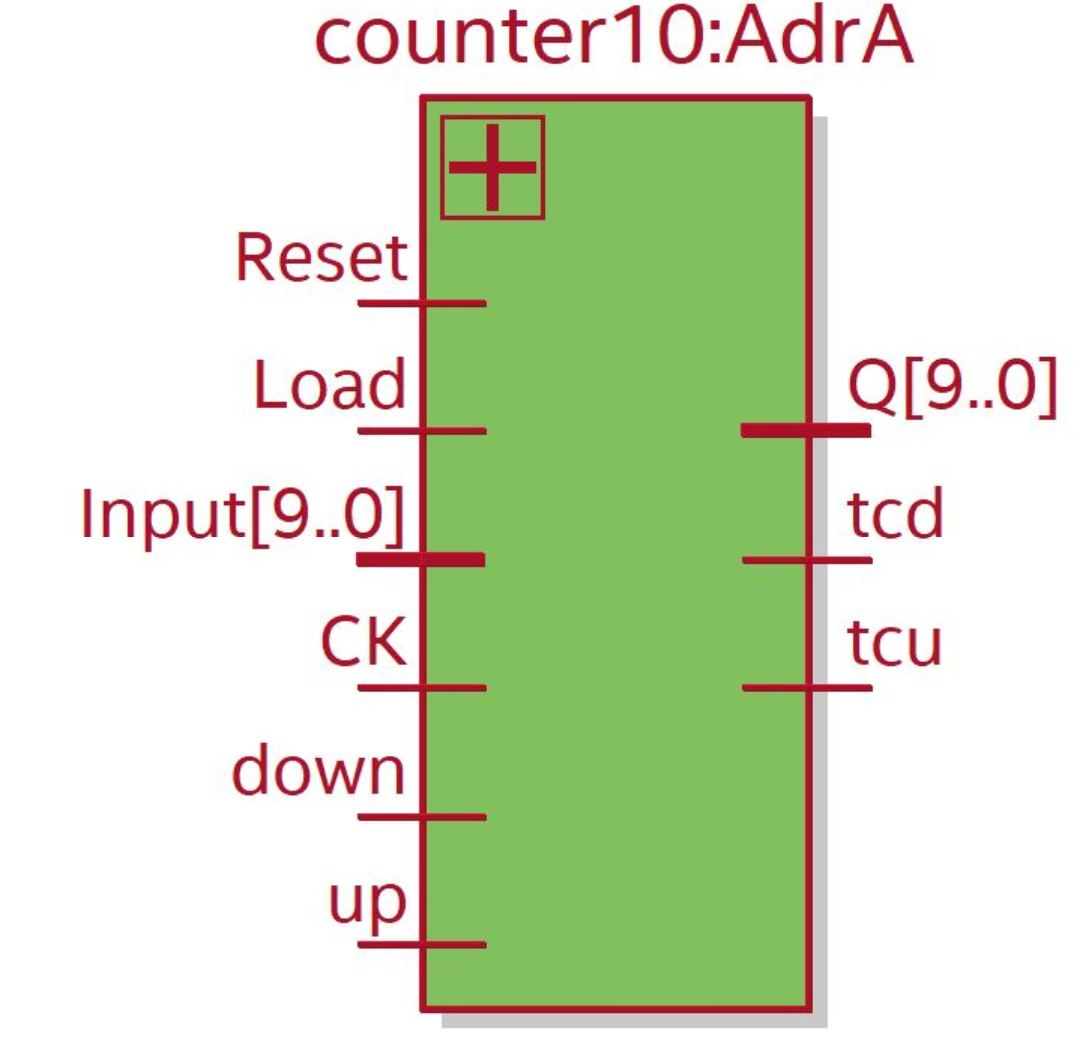
\includegraphics[scale = 0.47]{immagini/counter10.jpg}
	\caption{10 bit counter}
\end{figure}
The counter can count up or down. 
Furthermore, the output ports $tcd$ and $tcu$ have an high logical value when the counter reaches respectively its minimum or maximum possible value.

\begin{figure}[h]
	\centering
	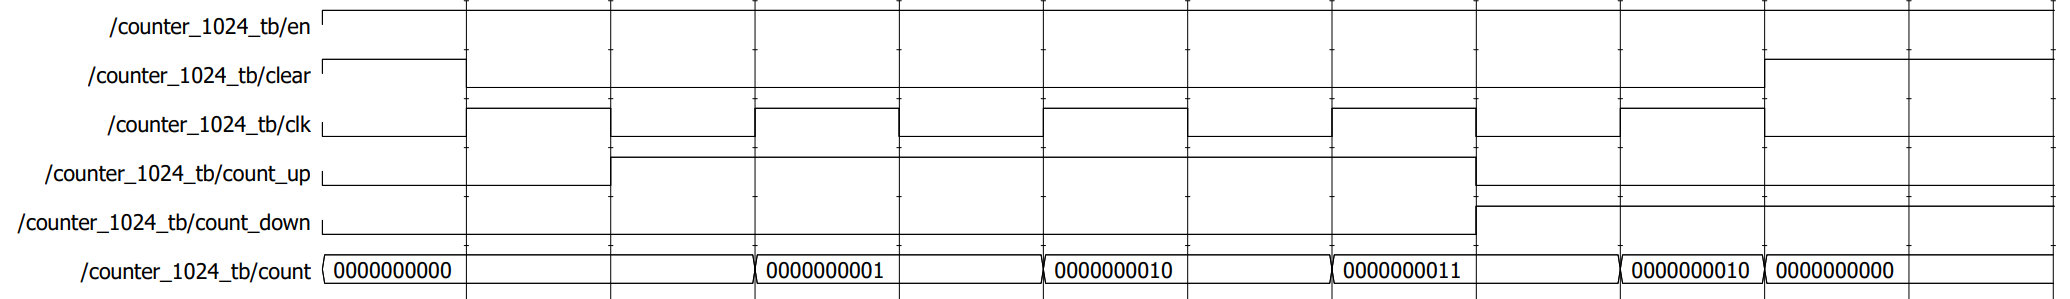
\includegraphics[scale = 0.47]{immagini/counter_tb.png}
	\caption{10 bit counter test bench}
\end{figure}





\end{document}




